% ============================================================
%  Artigo Técnico Red Hat
%  Argo CD Hub-and-Spoke: GitOps Orientado a Domínio no OpenShift no Bradesco
%  Engine: pdfLaTeX
% ============================================================
\documentclass[11pt,a4paper]{article}

% ── Encoding & fonts ────────────────────────────────────────
\usepackage[T1]{fontenc}
\usepackage[utf8]{inputenc}
\usepackage{lmodern}
\usepackage{microtype}

% ── Page geometry ───────────────────────────────────────────
\usepackage[
  top=25mm, bottom=25mm,
  left=25mm, right=25mm,
  headheight=14pt
]{geometry}

% ── Colors (Red Hat brand palette) ──────────────────────────
\usepackage[dvipsnames,svgnames,table]{xcolor}
\definecolor{rhred}{HTML}{EE0000}
\definecolor{rhdark}{HTML}{151515}
\definecolor{rhgray}{HTML}{6A6E73}
\definecolor{rhlightgray}{HTML}{F5F5F5}
\definecolor{rhblue}{HTML}{0066CC}
\definecolor{rhaccent}{HTML}{C9190B}

% ── Graphics & figures ──────────────────────────────────────
\usepackage{graphicx}
\usepackage{float}
\usepackage[labelfont=bf, font=small]{caption}
\usepackage{subcaption}
\graphicspath{{figures/}}

% ── Tables ──────────────────────────────────────────────────
\usepackage{booktabs}
\usepackage{tabularx}
\usepackage{multirow}
\usepackage{array}
\renewcommand{\arraystretch}{1.3}

% ── Code listings ───────────────────────────────────────────
\usepackage{listings}
\usepackage{lstautogobble}

\lstdefinestyle{yaml}{
  language=,
  basicstyle=\ttfamily\small,
  backgroundcolor=\color{rhlightgray},
  frame=single,
  framesep=4pt,
  rulecolor=\color{rhgray!40},
  breaklines=true,
  postbreak=\mbox{\textcolor{rhred}{$\hookrightarrow$}\space},
  keywordstyle=\color{rhred}\bfseries,
  stringstyle=\color{rhaccent},
  commentstyle=\color{rhgray}\itshape,
  numbers=left,
  numberstyle=\tiny\color{rhgray},
  numbersep=8pt,
  autogobble=true,
  tabsize=2,
  captionpos=b,
}

\lstdefinestyle{bash}{
  style=yaml,
  morekeywords={oc,kubectl,helm,kustomize,argocd,helm,helmfile},
}

\lstset{style=yaml}

% ── TikZ for architecture diagrams ──────────────────────────
\usepackage{tikz}
\usetikzlibrary{shapes.geometric, arrows.meta, positioning, fit, backgrounds, shadows.blur}

% ── Section styling ─────────────────────────────────────────
\usepackage{titlesec}
\titleformat{\section}
  {\color{rhdark}\large\bfseries}
  {\color{rhred}\thesection.}{0.6em}{}
  [\vspace{-2pt}\textcolor{rhred}{\rule{\linewidth}{0.4pt}}]

\titleformat{\subsection}
  {\color{rhdark}\normalsize\bfseries}
  {\color{rhgray}\thesubsection.}{0.5em}{}

\titleformat{\subsubsection}
  {\color{rhdark}\normalsize\itshape}
  {\thesubsubsection.}{0.4em}{}

% ── Header & footer ─────────────────────────────────────────
\usepackage{fancyhdr}
\pagestyle{fancy}
\fancyhf{}
\renewcommand{\headrulewidth}{0pt}
\fancyhead[L]{\small\color{rhgray}\textit{Red Hat --- Artigo Técnico}}
\fancyhead[R]{\small\color{rhgray}\textit{Argo CD Hub-and-Spoke: GitOps Orientado a Domínio}}
\fancyfoot[C]{\small\color{rhgray}\thepage}
\fancyfoot[R]{\small\color{rhgray}\textit{\today}}

% ── Hyperlinks ──────────────────────────────────────────────
\usepackage[
  colorlinks=true,
  linkcolor=rhred,
  urlcolor=rhred,
  citecolor=rhred,
  pdftitle={Argo CD Hub-and-Spoke: GitOps Orientado a Domínio no OpenShift no Bradesco},
  pdfauthor={Seu Nome},
  pdfsubject={GitOps, Argo CD, Hub-and-Spoke, OpenShift, Segregação por Domínio},
  pdfkeywords={argocd, hub-spoke, openshift, gitops, applicationset, path-generator}
]{hyperref}

% ── Bibliography ────────────────────────────────────────────
\usepackage[numbers,sort&compress]{natbib}
\bibliographystyle{plainnat}

% ── Misc helpers ────────────────────────────────────────────
\usepackage{enumitem}
\usepackage{parskip}
\setlength{\parskip}{6pt}
\usepackage{mdframed}
\usepackage{amsmath}

% ── Callout / info-box environment ──────────────────────────
\newmdenv[
  backgroundcolor=rhred!6,
  linecolor=rhred,
  linewidth=2pt,
  topline=false, rightline=false, bottomline=false,
  leftmargin=0pt, rightmargin=0pt,
  innerleftmargin=10pt, innerrightmargin=10pt,
  innertopmargin=6pt, innerbottommargin=6pt,
  skipabove=8pt, skipbelow=8pt,
]{infobox}

\newmdenv[
  backgroundcolor=rhaccent!6,
  linecolor=rhaccent,
  linewidth=2pt,
  topline=false, rightline=false, bottomline=false,
  leftmargin=0pt, rightmargin=0pt,
  innerleftmargin=10pt, innerrightmargin=10pt,
  innertopmargin=6pt, innerbottommargin=6pt,
  skipabove=8pt, skipbelow=8pt,
]{warnbox}

% ============================================================
\begin{document}

% ── Title page ──────────────────────────────────────────────
\begin{titlepage}
  \newgeometry{top=20mm,bottom=20mm,left=25mm,right=25mm}

  % Red Hat top bar
  \noindent\textcolor{rhred}{\rule{\linewidth}{4pt}}
  \vspace{4mm}

  \noindent
  \begin{minipage}[t]{0.15\linewidth}
    \textcolor{rhred}{\textbf{\Large RH}}
  \end{minipage}
  \hfill
  \begin{minipage}[t]{0.45\linewidth}
    \raggedleft\small\color{rhgray}
    Artigo Técnico\\
    OpenShift / GitOps
  \end{minipage}

  \vspace{30mm}

  {\color{rhred}\fontsize{28}{34}\selectfont\bfseries
    GitOps em Escala:\par
  }
  {\fontsize{18}{28}\selectfont\bfseries\color{rhdark}
    Arquitetura Argo~CD Hub-and-Spoke\par
    Orientada a Domínio no Red~Hat OpenShift no Bradesco\par
  }

  \vspace{8mm}
  \textcolor{rhgray}{\rule{0.4\linewidth}{0.8pt}}
  \vspace{6mm}

  {\large\color{rhgray}
    \textbf{Autores:} Seu Nome, Nome do Coautor\\[4pt]
    \textbf{Organização:} Sua Empresa / Red Hat Partner\\[4pt]
    \textbf{Data:} \today\\[4pt]
    \textbf{Versão:} 1.0
  }

  \vfill

  % Abstract box
  \noindent\colorbox{rhlightgray}{%
    \begin{minipage}{\linewidth}
      \vspace{6pt}
      \hspace{6pt}{\small\bfseries Resumo}\par
      \vspace{2pt}
      \hspace{6pt}\parbox{0.97\linewidth}{%
        \small
        Este artigo descreve a migração de uma topologia do Argo~CD por ambiente ---
        uma instância para cada um dos ambientes de desenvolvimento, staging e produção ---
        para uma arquitetura hub-and-spoke orientada a domínio no Red~Hat OpenShift.
        O modelo original concentrava todas as cargas de trabalho de aplicações de negócio
        em um único controlador do Argo~CD por ambiente, criando um gargalo de sincronização
        e falhas em cascata nos fluxos de GitOps.
        A solução introduz uma instância central de \emph{hub} do Argo~CD que provisiona
        instâncias \emph{spoke} do Argo~CD, delimitadas por domínio, por meio de path
        generators do \texttt{ApplicationSet}, apoiadas por um Helm chart padronizado com
        sub-charts e um registro de aplicações estruturado por caminho (path).
        O resultado são domínios de GitOps isolados por falha, escaláveis de forma
        independente, com um blast radius drasticamente reduzido em caso de falha de
        controlador.
      }
      \vspace{6pt}
    \end{minipage}%
  }

  \vspace{8mm}
  \noindent\textcolor{rhred}{\rule{\linewidth}{2pt}}
  \restoregeometry
\end{titlepage}

\tableofcontents
\newpage

% ============================================================
\section{Introdução}
\label{sec:intro}

Organizações de software modernas que operam no Red~Hat OpenShift costumam evoluir por
estágios previsíveis de adoção do GitOps.
O primeiro estágio é o GitOps ``centrado em ambiente'': uma única instância do Argo~CD
gerencia todas as aplicações destinadas a um determinado ambiente --- desenvolvimento,
staging e produção.

Esse modelo é fácil de entender inicialmente, mas entra em colapso sob o peso de um
portfólio de aplicações em crescimento, porque um único controlador passa a ser o domínio
de falha compartilhado por todos os domínios de negócio da organização.

Nossa organização atingiu esse ponto de inflexão quando a instância de produção do
Argo~CD começou a apresentar falhas sistemáticas de sincronização sob a carga combinada
de todas as cargas de trabalho de negócio.
Fluxos disparados por webhook, automações de image-updater e sincronizações manuais
disputavam a mesma fila de reconciliação, gerando timeouts em cascata difíceis de
atribuir a uma única equipe ou aplicação.

Este artigo documenta nossa migração para uma topologia \emph{hub-and-spoke orientada a
domínio}, na qual a instância hub do Argo~CD é responsável exclusivamente por provisionar
e manter as instâncias spoke do Argo~CD, cada uma delimitada a um único domínio de
negócio.
As aplicações são implantadas pela instância spoke do Argo~CD dona do domínio, e não por
um controlador compartilhado em nível de ambiente.

% ============================================================
\section{Definição do Problema}
\label{sec:problem}

\subsection{A topologia por ambiente e suas limitações}

O modelo de implantação original alocava uma instância do Argo~CD por ambiente:

\begin{itemize}[leftmargin=1.5em]
  \item \texttt{argocd-dev} --- gerenciava todas as aplicações do ambiente de
        desenvolvimento em todos os domínios de negócio.
  \item \texttt{argocd-staging} --- mesmo escopo para o ambiente de staging.
  \item \texttt{argocd-prod} --- mesmo escopo para o ambiente de produção.
\end{itemize}

Cada instância era configurada de forma idêntica e mantida de maneira independente.
À medida que o número de aplicações e equipes crescia, diversas fragilidades estruturais
foram surgindo.

\subsection{Modos de falha observados}

\begin{description}[leftmargin=0pt, style=nextline]
  \item[\textbf{Gargalo de reconciliação.}]
    Todos os domínios compartilhavam um único \texttt{argocd-application-controller}.
    Durante horários de pico --- deploy trains, releases de sprint, promoções em lote
    durante a madrugada --- a profundidade da fila de reconciliação disparava, atrasando
    a conclusão das sincronizações em até 40 minutos.

  \item[\textbf{Falhas de sincronização em cascata.}]
    Uma \texttt{Application} com comportamento problemático em um domínio (por exemplo,
    um ConfigMap muito grande causando timeout no diff de server-side apply) bloqueava a
    reconciliação de domínios sem nenhuma relação entre si, violando o princípio de
    isolamento de falhas.

  \item[\textbf{Quebra na integração dos fluxos de trabalho.}]
    Pipelines de CI/CD que chamavam \texttt{argocd app sync} com
    \texttt{--timeout} passaram a apresentar falhas espúrias, porque o controlador
    estava ocupado atendendo outros tenants.
    Isso corroeu a confiança no GitOps como uma primitiva de entrega confiável.
\end{description}

\subsection{Requisitos para o novo modelo}

A Tabela~\ref{tab:requirements} lista os requisitos que orientaram a decisão
arquitetural.

\begin{table}[H]
  \centering
  \caption{Requisitos para a arquitetura de GitOps orientada a domínio}
  \label{tab:requirements}
  \small
  \begin{tabularx}{\linewidth}{@{} l l X @{}}
    \toprule
    \textbf{ID} & \textbf{Categoria} & \textbf{Requisito} \\
    \midrule
    R-01 & Isolamento     & Uma falha no Argo~CD de um domínio não deve afetar outros domínios \\
    R-02 & Escalabilidade & Adicionar um novo domínio não deve exigir mudanças nas instâncias existentes \\
    R-03 & Padronização   & Todas as instâncias spoke devem compartilhar uma configuração base comum \\
    R-04 & Automação      & O provisionamento dos spokes deve ser totalmente orientado por GitOps (sem etapas manuais) \\
    R-05 & Observabilidade& O status de sincronização deve ser visível por domínio e por ambiente \\
    R-06 & DR             & Uma falha no hub não deve afetar reconciliações de spokes em andamento \\
    \bottomrule
  \end{tabularx}
\end{table}

% ============================================================
\section{Arquitetura da Solução}
\label{sec:architecture}

\subsection{Visão geral do hub-and-spoke orientado a domínio}

A nova topologia substitui as três instâncias compartilhadas por ambiente por uma
hierarquia de dois níveis: uma única instância \emph{hub} do Argo~CD, dona do ciclo de
vida das instâncias \emph{spoke} do Argo~CD, cada uma delimitada a um domínio de negócio.

\begin{itemize}[leftmargin=1.5em]
  \item \textbf{Hub Argo~CD} --- reside no cluster OpenShift do hub.
        Sua única responsabilidade é implantar e reconciliar as instâncias spoke do
        Argo~CD (e seus recursos de suporte) a partir do repositório de Helm chart.
        Ele \emph{não} implanta aplicações de negócio diretamente.

  \item \textbf{Spoke Argo~CD (por domínio)} --- uma instância por domínio de negócio,
        implantada no cluster apropriado.
        Cada instância spoke gerencia apenas as aplicações pertencentes ao seu domínio,
        lendo do repositório de aplicações sob o caminho (path) correspondente ao
        domínio.
\end{itemize}

A Figura~\ref{fig:hub-spoke} mostra a arquitetura lógica.

% ── TikZ architecture diagram ───────────────────────────────
\begin{figure}[H]
\centering
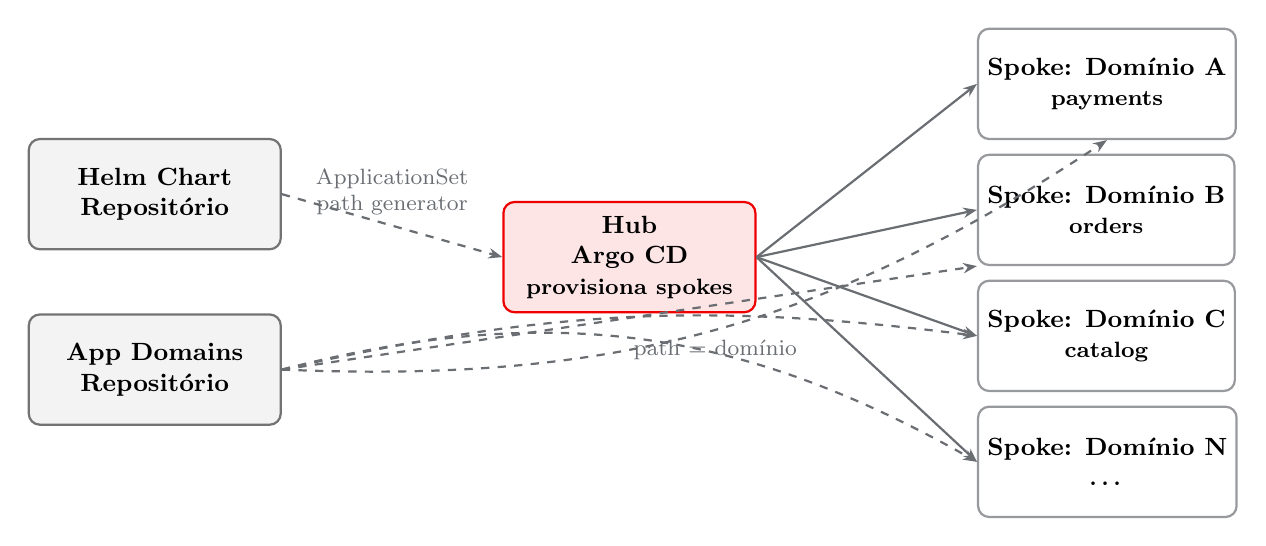
\begin{tikzpicture}[
  node distance=10mm and 20mm,
  box/.style={
    draw=rhgray, rounded corners=4pt, thick,
    minimum width=32mm, minimum height=14mm,
    fill=rhlightgray, font=\small\bfseries, align=center
  },
  hub/.style={box, draw=rhred, fill=rhred!10},
  spoke/.style={box, draw=rhgray!70, fill=white},
  repo/.style={box, draw=rhdark!60, fill=rhdark!5},
  arrow/.style={-{Stealth[length=5pt]}, thick, rhgray},
  darrow/.style={arrow, dashed},
  lbl/.style={font=\footnotesize\color{rhgray}, align=center}
]

% Repositories
\node[repo] (helm-repo)  {Helm Chart\\Repositório};
\node[repo, below=8mm of helm-repo] (apps-repo) {App Domains\\Repositório};

% Hub
\node[hub, right=28mm of helm-repo, yshift=-8mm] (hub)
  {Hub\\Argo~CD\\{\footnotesize provisiona spokes}};

% Spokes
\node[spoke, right=28mm of hub, yshift=22mm]  (s1)
  {Spoke: Domínio A\\{\footnotesize payments}};
\node[spoke, right=28mm of hub, yshift=6mm]   (s2)
  {Spoke: Domínio B\\{\footnotesize orders}};
\node[spoke, right=28mm of hub, yshift=-10mm] (s3)
  {Spoke: Domínio C\\{\footnotesize catalog}};
\node[spoke, right=28mm of hub, yshift=-26mm] (s4)
  {Spoke: Domínio N\\{\footnotesize \ldots}};

% Hub reads Helm chart repo
\draw[darrow] (helm-repo.east) -- node[above,lbl]{ApplicationSet\\path generator} (hub.west);

% Hub deploys spokes
\draw[arrow] (hub.east) -- (s1.west);
\draw[arrow] (hub.east) -- (s2.west);
\draw[arrow] (hub.east) -- (s3.west);
\draw[arrow] (hub.east) -- (s4.west);

% Spokes read App Domains
\draw[darrow, bend right=18] (apps-repo.east) to node[below,lbl]{path = domínio} (s1.south);
\draw[darrow] (apps-repo.east) -- (s2.south west);
\draw[darrow, bend left=10] (apps-repo.east) to (s3.west);
\draw[darrow, bend left=22] (apps-repo.east) to (s4.west);

\end{tikzpicture}
\caption{Hub-and-spoke orientado a domínio: o hub Argo~CD implanta as instâncias spoke
  a partir do repositório de Helm chart; cada spoke lê suas aplicações a partir do
  repositório App Domains, no caminho (path) correspondente ao seu domínio.}
\label{fig:hub-spoke}
\end{figure}

\subsection{Mapeamento de componentes}

\begin{table}[H]
  \centering
  \caption{Papel de cada componente na arquitetura orientada a domínio}
  \label{tab:components}
  \small
  \begin{tabularx}{\linewidth}{@{} l l X @{}}
    \toprule
    \textbf{Componente} & \textbf{Camada} & \textbf{Papel} \\
    \midrule
    Hub Argo~CD
      & Plano de controle
      & Provisiona e reconcilia todas as instâncias spoke do Argo~CD; não é dono de
        nenhuma aplicação de negócio \\
    \texttt{ApplicationSet} (hub)
      & Automação
      & Usa um path generator sobre o repositório de Helm chart para criar uma
        \texttt{Application} de spoke para cada diretório de domínio descoberto \\
    Repositório de Helm Chart
      & Padronização
      & Umbrella chart com sub-charts que definem a configuração canônica do hub e dos
        spokes do Argo~CD; versionado e compartilhado entre todos os domínios \\
    Repositório App Domains
      & Inventário de aplicações
      & Lista de aplicações estruturada por caminho (path); cada diretório de nível
        superior é um domínio; cada Argo~CD spoke aponta para seu próprio diretório \\
    Spoke Argo~CD (por domínio)
      & Entrega
      & Implanta e reconcilia as aplicações declaradas em seu path de domínio;
        controlador, fila e RBAC isolados \\
    \texttt{ApplicationSet} (spoke)
      & Automação
      & Usa um path generator sobre o App Domains para criar uma \texttt{Application}
        para cada serviço declarado dentro do domínio \\
    \bottomrule
  \end{tabularx}
\end{table}

\subsection{Estrutura dos repositórios}

A arquitetura se apoia em três repositórios Git com responsabilidades claramente
separadas.

% \subsubsection{Repositório 1 --- Helm chart (padronização de hub e spoke)}

% Este repositório contém o umbrella chart do Helm que empacota as configurações do
% hub e dos spokes do Argo~CD como sub-charts.
% Ele é a fonte única de verdade para a versão do Argo~CD, requests de recursos,
% templates de RBAC e defaults operacionais em todas as instâncias.

% /*
% \begin{lstlisting}[style=bash, numbers=none,
%   caption={Layout do repositório de Helm chart},
%   label={lst:helm-repo}]
% argo-helm-charts/
% ├── Chart.yaml                  # umbrella chart
% ├── values.yaml                 # defaults globais
% ├── values-hub.yaml             # overrides específicos do hub
% ├── charts/
% │   ├── argocd-hub/             # sub-chart: configuração da instância hub
% │   │   ├── Chart.yaml
% │   │   ├── values.yaml
% │   │   └── templates/
% │   │       ├── argocd.yaml     # ArgoCD CR (OpenShift GitOps)
% │   │       └── applicationset-spokes.yaml
% │   └── argocd-spoke/           # sub-chart: template da instância spoke
% │       ├── Chart.yaml
% │       ├── values.yaml         # defaults do spoke (replicas, QPS, …)
% │       └── templates/
% │           ├── argocd.yaml
% │           ├── appproject.yaml
% │           └── applicationset-apps.yaml
% └── domains/
%     ├── payments/
%     │   └── values.yaml         # overrides específicos do domínio
%     ├── orders/
%     │   └── values.yaml
%     └── catalog/
%         └── values.yaml
% \end{lstlisting}

% \subsubsection{Repositório 2 --- Registro de aplicações}

% Este repositório contém os manifests de aplicação de cada domínio de negócio.
% A hierarquia de diretórios espelha a topologia dos spokes: o caminho de nível
% superior é o nome do domínio, e os subcaminhos representam serviços individuais
% ou grupos de aplicações.

% \begin{lstlisting}[style=bash, numbers=none,
%   caption={Layout do repositório de registro de aplicações},
%   label={lst:apps-repo}]
% argo-apps/
% ├── payments/
% │   ├── payment-gateway/
% │   │   └── application.yaml
% │   ├── fraud-detection/
% │   │   └── application.yaml
% │   └── ledger/
% │       └── application.yaml
% ├── orders/
% │   ├── order-api/
% │   │   └── application.yaml
% │   └── fulfillment/
% │       └── application.yaml
% └── catalog/
%     ├── product-service/
%     │   └── application.yaml
%     └── search-indexer/
%         └── application.yaml
% \end{lstlisting}

% \subsubsection{Repositório 3 --- Código-fonte das aplicações (por serviço)}

% Cada serviço mantém seus próprios Helm charts ou overlays de Kustomize em
% repositórios dedicados ou em um monorepo compartilhado.
% Esses repositórios são referenciados pelas entradas \texttt{application.yaml}
% no App Domains e, fora isso, são invisíveis para as instâncias hub ou spoke
% do Argo~CD.

\subsection{Decisões de projeto}

\begin{description}[leftmargin=0pt, style=nextline]
  \item[\textbf{Domínio como limite de isolamento, não ambiente:}]
    Os ambientes (dev, staging, prod) são expressos como values do Helm ou overlays do
    Kustomize dentro do spoke de cada domínio, e não como instâncias separadas do
    Argo~CD.
    Isso preserva a simplicidade operacional ao mesmo tempo em que atinge o isolamento
    de falhas no nível do domínio de negócio --- o limite que realmente importa para a
    resposta a incidentes.

  \item[\textbf{O hub Argo~CD gerencia apenas os spokes:}]
    Manter as aplicações de negócio fora do escopo de reconciliação do hub evita a
    saturação do hub e faz com que a saúde do hub esteja diretamente correlacionada à
    disponibilidade dos spokes.
    Se o hub estiver degradado, os spokes em execução continuam reconciliando suas
    aplicações sem interrupção (R-06).

  \item[\textbf{Path generator em vez de cluster/list generators:}]
    O path generator do tipo \texttt{git} descobre novos domínios automaticamente
    quando um novo diretório é adicionado à árvore \texttt{domains/} do repositório de
    Helm chart ou ao App Domains.
    Isso atende aos requisitos R-02 e R-04 sem exigir qualquer alteração nos manifests
    de \texttt{ApplicationSet} existentes.

  \item[\textbf{Sub-charts para padronização:}]
    Codificar a configuração do Argo~CD em um sub-chart compartilhado do Helm (em vez
    de YAML bruto por domínio) garante que uma única versão do chart
    \texttt{argocd-spoke} fixe a release do Argo~CD para todos os spokes
    simultaneamente, transformando upgrades em uma operação de um único commit (R-03).
\end{description}

% ============================================================
\section{Implementação}
\label{sec:implementation}

\subsection{Pré-requisitos}

\begin{itemize}[leftmargin=1.5em]
  \item Red~Hat OpenShift no cluster do hub (versão \textit{X.Y})
  \item OpenShift GitOps Operator instalado no hub (provisiona o hub Argo~CD)
  \item O cluster do hub possui conectividade de rede com os API servers de todos os
        clusters spoke
  \item Os três repositórios Git estão acessíveis a partir do cluster do hub
  \item Helm \textit{X.Y} disponível no ambiente de CI para lint e testes dos charts
\end{itemize}

\subsection{Instalando o hub Argo~CD}


\subsection{ApplicationSet --- provisionando instâncias spoke}

O hub Argo~CD usa um path generator do tipo \texttt{git} que varre o diretório
\texttt{domains/} do repositório de Helm chart.
Cada subdiretório descoberto se torna uma \texttt{Application} que implanta o sub-chart
\texttt{argocd-spoke} com o override de values daquele domínio.

\begin{lstlisting}[style=yaml,
  caption={ApplicationSet do hub: path generator sobre o repositório de Helm chart},
  label={lst:hub-appset}]
apiVersion: argoproj.io/v1alpha1
kind: ApplicationSet
metadata:
  name: spoke-provisioner
  namespace: openshift-gitops
spec:
  goTemplate: true
  goTemplateOptions: ["missingkey=error"]
  generators:
    - git:
        repoURL: https://github.com/<org>/argo-helm-charts.git
        revision: HEAD
        directories:
          - path: domains/*
  template:
    metadata:
      name: "spoke-{{ .path.basename }}"
    spec:
      project: default
      source:
        repoURL: https://github.com/<org>/argo-helm-charts.git
        targetRevision: HEAD
        path: "."
        helm:
          releaseName: "argocd-{{ .path.basename }}"
          valueFiles:
            - values.yaml
            - "domains/{{ .path.basename }}/values.yaml"
      destination:
        server: https://kubernetes.default.svc
        namespace: "argocd-{{ .path.basename }}"
      syncPolicy:
        automated:
          prune: true
          selfHeal: true
        syncOptions:
          - CreateNamespace=true
          - ServerSideApply=true
\end{lstlisting}

\begin{infobox}
  \textbf{Como novos domínios são integrados (onboarding).}
  Adicionar um novo domínio de negócio requer apenas duas etapas: (1)~criar
  \texttt{domains/<novo-domínio>/values.yaml} no repositório de Helm chart, e
  (2)~criar o diretório de nível superior correspondente no repositório App Domains.
  O \texttt{ApplicationSet} do hub detecta o novo path dentro de
  \texttt{requeueAfterSeconds} e provisiona o spoke automaticamente.
  Nenhuma alteração nos manifests existentes é necessária.
\end{infobox}

\subsection{Sub-chart do Helm: argocd-spoke}


\subsection{ApplicationSet do spoke --- implantando aplicações do domínio}

Cada instância spoke do Argo~CD contém um único \texttt{ApplicationSet}, gerado pelo
sub-chart \texttt{argocd-spoke}.
Ele usa um path generator do tipo \texttt{git} sobre o repositório App Domains,
delimitado à subárvore do domínio.

\begin{lstlisting}[style=yaml,
  caption={Template do ApplicationSet do spoke dentro do sub-chart argocd-spoke},
  label={lst:spoke-appset}]
apiVersion: argoproj.io/v1alpha1
kind: ApplicationSet
metadata:
  name: {{ .Values.domain.name }}-apps
  namespace: {{ .Release.Namespace }}
spec:
  goTemplate: true
  generators:
    - git:
        repoURL: https://github.com/<org>/argo-apps.git
        revision: HEAD
        directories:
          - path: "{{ .Values.domain.name }}/*"
  template:
    metadata:
      name: "{{ `{{ .path.basename }}` }}"
    spec:
      project: {{ .Values.domain.name }}
      source:
        repoURL: "{{ `{{ index .path.segments 1 | printf \"https://github.com/<org>/%s\" }}` }}"
        targetRevision: HEAD
        path: "."
      destination:
        server: https://kubernetes.default.svc
        namespace: "{{ `{{ .path.basename }}` }}"
      syncPolicy:
        automated:
          prune: true
          selfHeal: true
        syncOptions:
          - CreateNamespace=true
          - ServerSideApply=true
\end{lstlisting}

% ============================================================
\section{Desafios e Mitigações}
\label{sec:challenges}

\subsection{Desafio 1: Migração sem downtime}

\subsection{Desafio 2: Reconciliação do ApplicationSet do hub durante importação em massa de domínios}

\subsection{Desafio 3: Herança de values entre sub-charts do Helm}

\subsection{Desafio 4: Bootstrapping de RBAC do Argo~CD spoke}

% ============================================================
\section{Resultados e Conclusões}
\label{sec:results}

% ============================================================
\section{Lições Aprendidas}
\label{sec:lessons}

\begin{enumerate}[leftmargin=1.5em, label=\textbf{L-\arabic*.}]
  \item \textbf{Isole por domínio de falha, não por ambiente.}
    O eixo de ambiente (dev/staging/prod) é uma preocupação de implantação, tratada por
    overlays de values.
    O eixo de isolamento de falhas é o domínio de negócio --- o limite ao longo do qual
    as equipes são donas de seus SLAs.
    Alinhar as instâncias do Argo~CD aos domínios de negócio mapeia diretamente o
    escopo do controlador à responsabilidade por incidentes.

  \item \textbf{O hub não deve hospedar cargas de trabalho de negócio.}
    Qualquer \texttt{Application} de negócio no hub acopla sua superfície de falha ao
    plano de provisionamento dos spokes.
    Mantenha a lista de \texttt{Application} do hub populada exclusivamente pelo
    \texttt{spoke-provisioner}.

  \item \textbf{Sub-charts do Helm são a abstração correta para padronização entre
        múltiplas instâncias.}
    Uma versão compartilhada de sub-chart é uma garantia mais forte de paridade de
    configuração do que convenções documentadas ou YAML copiado e colado.
    Invista cedo em \texttt{values.schema.json} para expor erros em tempo de lint, e
    não em tempo de execução.

  \item \textbf{Path generators escalam melhor do que cluster/list generators para
        cargas de trabalho homogêneas.}
    Adicionar um domínio é uma operação de sistema de arquivos (criar um diretório).
    Não há registro, ConfigMap ou configuração de generator para atualizar.
    A abordagem de convenção sobre configuração rende juros compostos à medida que o
    número de domínios cresce.

  \item \textbf{Migre um domínio de cada vez, com a sincronização desabilitada.}
    A migração em três fases (desabilitar, espelhar, cut over) é mais lenta do que uma
    importação em massa, mas elimina o risco de uma dupla sincronização que derrube
    temporariamente um serviço em produção.
    Automatize a sequência de fases em um script e exija um gate de aprovação via PR
    entre as fases.
\end{enumerate}

% ============================================================
\section{Conclusão}
\label{sec:conclusion}

A migração do modelo por ambiente para o hub-and-spoke do Argo~CD orientado a domínio
resolveu os dois problemas operacionais mais críticos: a saturação de reconciliação e o
blast radius entre domínios.
Ao atribuir a cada domínio de negócio o seu próprio controlador do Argo~CD ---
provisionado automaticamente pelo hub por meio de um path generator de
\texttt{ApplicationSet} e padronizado por um sub-chart compartilhado do Helm --- a
equipe de plataforma eliminou tanto o domínio de falha compartilhado quanto o esforço
manual de onboarding que se acumulava no modelo antigo.

Para equipes que consideram essa mesma jornada, a constatação mais importante é que a
unidade natural de isolamento no GitOps não é o ambiente de implantação, e sim o limite
organizacional --- a equipe ou o domínio responsável pela resposta a incidentes.
Construir a topologia do Argo~CD alinhada a esse limite torna o sistema ao mesmo tempo
mais resiliente e mais compreensível.

% ============================================================
\section*{Agradecimentos}
\addcontentsline{toc}{section}{Agradecimentos}

Os autores agradecem às equipes de engenharia do Red Hat OpenShift e GitOps pela
documentação e pelo suporte da comunidade ao longo desta implementação.

% ============================================================
\section*{Referências}
\addcontentsline{toc}{section}{Referências}

\begin{thebibliography}{99}
\bibitem{argocd-docs}
  Argo~CD. \textit{Argo CD --- Declarative GitOps CD for Kubernetes}.
  \url{https://argo-cd.readthedocs.io}

\bibitem{appset-docs}
  Argo~CD. \textit{ApplicationSet Controller --- Git Generator}.
  \url{https://argocd-applicationset.readthedocs.io/en/stable/Generators-Git/}

\bibitem{openshift-gitops}
  Red Hat. \textit{OpenShift GitOps Operator Documentation}.
  \url{https://docs.openshift.com/gitops}

\bibitem{helm-subchart}
  Helm. \textit{Chart Dependencies (Sub-charts)}.
  \url{https://helm.sh/docs/chart_template_guide/subcharts_and_globals/}

\bibitem{cncf-gitops}
  OpenGitOps. \textit{GitOps Principles v1.0}.
  Cloud Native Computing Foundation, 2021.

\bibitem{argo-best-practices}
  Argo~CD. \textit{Best Practices}.
  \url{https://argo-cd.readthedocs.io/en/stable/user-guide/best_practices/}
\end{thebibliography}

\end{document}
